\section{Experiments}
\label{sec:experiments}
\subsection{Evaluation Setup}
We evaluate LLaVA-3D-7B and 3D-LLaVA-7B-LoRA on one H100 80GB. QA uses greedy decoding, beam 1, with runner-matched prompts and inputs. ScanQA validation contains 4675 questions in 71 scenes and informed configuration selection. Its 500-question exploratory subset spans all 71 scenes; neither it nor the full-set sweeps provides an independent holdout. SQA3D~\citep{ma2023sqa3d} test contains 3519 questions in 67 scenes and was also inspected previously. \Cref{tab:evidence_map} summarizes the evidence; the supplement documents protocols, provenance, and reproduction limitations.

\begin{table}[t]
\centering
\small
\caption{\textbf{What each comparison tests.}}
\label{tab:evidence_map}
\setlength{\tabcolsep}{3pt}
\begin{tabular}{@{}p{0.24\columnwidth}p{0.71\columnwidth}@{}}
\toprule
Question & Comparison \\
\midrule
Deletion depth & Same token set removed at three layers (\cref{tab:fixedset}). \\
Retention & Early vs.\ late at matched analytical LM cost (\cref{tab:costmatched}). \\
Transfer & Fixed schedule vs.\ native, not early pruning (\cref{fig:transfereffects}). \\
Timing & GeoGate vs.\ native on one H100 (\cref{tab:efficiency}). \\
\bottomrule
\end{tabular}
\end{table}

Each comparison uses a matched native (unpruned) baseline from the same runner, listed in its table and the supplementary protocol index. We interpret results within runners, without combining different native baselines or quality and timing from separate runs.

\textbf{Selection and testing.} Exploratory ScanQA profiles informed L14, and joint validation point estimates selected R10. Fixed-set, paired-replay, and SQA3D/MMScan protocols were specified before their respective outcomes, but after the initial exploration. The SQA3D remainder fold was planned after the first fold's negative result. The onset rule, SQA3D R20 follow-up, profile-to-quality analysis, and throughput exclusions are post hoc. The supplement details the selection and testing chronology.

We report exact match (EM@1), consensus-based image description evaluation (CIDEr)~\citep{vedantam2015cider}, and mean intersection over union (mIoU). EM and mIoU use 0--100 scales; CIDEr differences use score points. For quality differences, the scene bootstrap resamples scenes with replacement, preserves paired questions, and computes a question-weighted mean. Reference-corpus inverse document frequency (IDF) remains fixed during CIDEr resampling. An interval containing zero does not by itself establish equivalence or non-inferiority; either claim requires a prespecified margin and an appropriate decision rule. Prespecified contrasts remain conditional on configuration selection; local max-$t$ corrections do not cover the historical search. Scene-ID checks find no overlap between the released-860K mixture and the ScanQA/SQA3D splits used here. The release lacks a complete historical training manifest.

\subsection{Token Selection and Deletion Depth}
\textbf{When each layer selects its own set.} On LLaVA-3D ScanQA validation, we delete the highest-attention 10\% of spatial tokens at L8, L14, or L20 and score the complete answer. Relative to random deletion at the same layer, top-set deletion costs an extra 0.29, 3.49, and 0.51 EM points, respectively. The L14-minus-L8 and L14-minus-L20 contrasts are $+3.20$ $[1.80,4.73]$ and $+2.97$ $[1.83,4.22]$ (97.5\% scene intervals). L14 has the largest excess loss, but each layer deletes different tokens.

\begin{table}[t]
\centering
\caption{\textbf{Same tokens, different deletion depths.} On LLaVA-3D ScanQA validation (4675 questions, 71 scenes), each row fixes the top 10\% of spatial tokens from one source layer. Entries compare EM loss relative to native: positive values mean greater loss at L14. Brackets give 97.5\% scene intervals.}
\label{tab:fixedset}
\resizebox{\columnwidth}{!}{%
\begin{tabular}{lcc}
\toprule
Source set & L14 minus L8 & L14 minus L20 \\
\midrule
L8  & $-0.26$ $[-0.70,0.19]$ & $+0.15$ $[-0.19,0.51]$ \\
L14 & $-1.50$ $[-2.29,-0.70]$ & $+2.63$ $[1.60,3.77]$ \\
L20 & $-1.30$ $[-2.03,-0.59]$ & $+2.16$ $[1.29,3.15]$ \\
\bottomrule
\end{tabular}}
\end{table}

\textbf{When token identity stays fixed.} We delete each source set at all three depths, holding the input, prompt, budget, seed, and native baseline fixed (\cref{tab:fixedset}). For the L14-selected set, deleting at L8 rather than L14 costs a further 1.50 EM points. The L20-selected set shows the same ordering (1.30 points). For both sets, deleting at L14 also hurts more than deleting at L20. Neither contrast is resolved for the L8-selected set. The prespecified criterion required L14 to cause greater damage than both other depths for at least two source sets; none qualifies. Thus deletion depth matters, but the peak under layer-specific selection does not identify L14 as the most damaging location. Fixed-set damage is measured against native, whereas the preceding contrasts measure excess damage over random deletion; subtracting them would not isolate a token-identity effect.

\textbf{Deleting a set is not the same as retaining it.} Deleting the top 10\% tests what is lost; it does not test whether the same 10\% suffices on its own. On 3D-LLaVA we test both directions at L14. Keeping ten top-ranked tokens gives 27.83 EM, versus $23.87\pm0.07$ for random and 23.51 for bottom-ranked tokens. Deleting those ten gives 23.81 EM, versus $27.79\pm0.12$ and 28.09, respectively (random: mean and sample standard deviation over three frozen seeds). This comparison favors the top-ranked set over those controls at L14; it does not compare a fixed retained set across depths.

\subsection{Retention at Matched Cost or Token Count}
\begin{table}[t]
\centering
\caption{\textbf{LLaVA-3D ScanQA validation schedule grid.} All 4675 questions are evaluated; GeoGate uses L14/R10. KV and FLOPs estimate LM cost, not total memory or latency.}
\label{tab:scanqa}
\resizebox{\columnwidth}{!}{%
\begin{tabular}{lcccccc}
\toprule
Method & Layer & Kept & EM@1 & CIDEr & Prompt KV & FLOPs \\
\midrule
Baseline & --- & 100\% & 27.34 & 93.96 & 100\% & 100\% \\
FastV-style & 2 & 50\% & 26.55 & 90.44 & 56.4\% & 59.2\% \\
\textbf{GeoGate} & 14 & 10\% & 27.79 & 94.33 & 21.5\% & 57.9\% \\
\bottomrule
\end{tabular}}
\end{table}

Late pruning produces ScanQA point estimates close to native, with uncertainty permitting both gains and losses. In \Cref{tab:scanqa}, R10 changes EM by $+0.45$ points (scene 95\% CI $[-0.07,0.99]$) and CIDEr by $+0.37$ ($[-1.14,1.89]$). These intervals establish neither improvement nor equivalence. The FastV-style L2/R50 control has similar analytical cost; this limited comparison does not characterize a complete Pareto frontier. PyramidDrop-style and AdaToken-inspired controls yield 27.25 and 26.95 EM, with paired results and approximation details in the supplement.

\begin{table}[t]
\centering
\caption{\textbf{LLaVA-3D ScanQA analytical-cost controls.} A separate validation runner adjusts early-layer budgets to input length to match L14/128 LM cost.}
\label{tab:costmatched}
\resizebox{\columnwidth}{!}{%
\begin{tabular}{lccc}
\toprule
Condition & Mean spatial tokens & EM@1 & CIDEr \\
\midrule
Native & 1463.96 & 27.42 & 94.06 \\
L2 cost matched & 699.71 & 26.67 & 90.67 \\
L8 cost matched & 491.79 & 26.87 & 92.27 \\
\textbf{L14/128} & 128.00 & 27.89 & 94.07 \\
\bottomrule
\end{tabular}}
\end{table}

On the LLaVA-3D ScanQA validation split used for selection, L14/128 outperforms L2 and L8 at matched analytical LM cost (\cref{tab:costmatched}). The early schedules retain about 700 and 492 spatial tokens on average, respectively. With shared input embeddings, L14 leads by 1.22 EM points over L2 $[0.42,2.12]$ and 1.03 over L8 $[0.24,1.85]$ (prespecified 97.5\% scene intervals). The budgets match estimated computation, not measured latency.

\begin{figure*}[t]
\centering
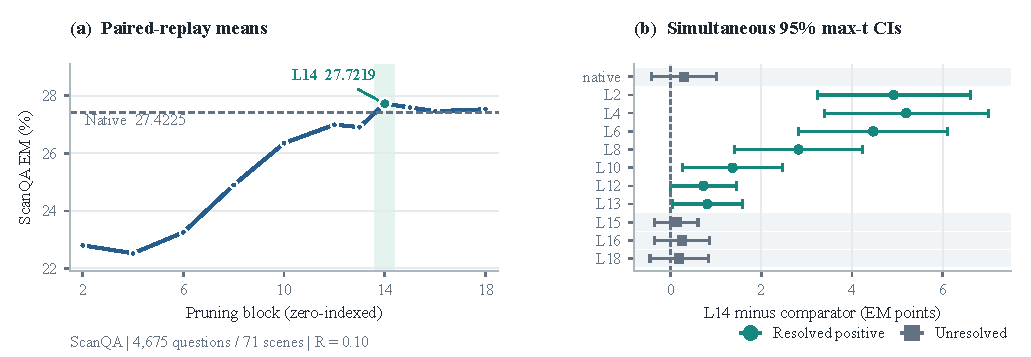
\includegraphics[width=\textwidth]{fig_layer_replay_paired_final.pdf}
\caption{\textbf{LLaVA-3D shared-input layer replay on ScanQA validation.} 4675 questions, 71 scenes, $R=0.10$. (a) Replay EM means with the runner's own native baseline. (b) All eleven L14-versus-comparator effects with frozen 95\% simultaneous scene-clustered max-$t$ intervals. These intervals cover the stated contrasts, not the historical configuration search. The original aggregate curve is reported separately in the supplement.}
\label{fig:layercurve}
\end{figure*}

Fixing the \emph{retention fraction} instead of the analytical cost answers a different question (\cref{fig:layercurve}). At 10\% retention on shared inputs, L14 exceeds L2/L4/L6/L8/L10/L12/L13, but the simultaneous contrasts do not distinguish L14 from L15/L16/L18 or from native (L14 minus native: $+0.2995$ EM $[-0.4100,1.0089]$). The evidence favors a late range over the specified early settings, not a unique optimum. The schedule grid likewise shows no resolved advantage for the 10\% budget over 5\% or 20\%.

\begin{table}[t]
\centering
\caption{\textbf{LLaVA-3D ScanQA comparison with official 3DZip.} Full validation set; compressed arms retain 128 spatial tokens, with GeoGate pruning after L14. Equal counts do not imply equal computation.}
\label{tab:official128}
\resizebox{\columnwidth}{!}{%
\begin{tabular}{lccc}
\toprule
Condition & Visual tokens & EM@1 & CIDEr \\
\midrule
Native & 1464.0 avg. & 27.23 & 93.48 \\
Official 3DZip & 128 & 25.05 & 86.02 \\
\textbf{GeoGate} & 128 & 27.96 & 94.25 \\
\bottomrule
\end{tabular}}
\end{table}

At an equal final count of 128 spatial tokens, GeoGate scores higher than official 3DZip on the inspected ScanQA validation split (\cref{tab:official128}): $+2.91$ EM $[1.96,3.90]$ and $+8.24$ CIDEr $[5.80,10.72]$ (95\% scene intervals). Against native the differences are $+0.73$ EM $[0.22,1.24]$ and $+0.77$ CIDEr $[-0.68,2.23]$. We use official 3DZip commit \texttt{2fec4a5}, identical RGB-D tensors, prompt and per-query seed, and cyclic condition order. Native and GeoGate share the expanded embedding and cap choices. GeoGate still processes the full sequence through L14. This is a quality comparison at equal final token count, not a comparison at equal computation or measured latency. \Cref{sec:supp_repro_index} identifies the available records and the missing historical runner version.

\begin{figure*}[t]
\centering
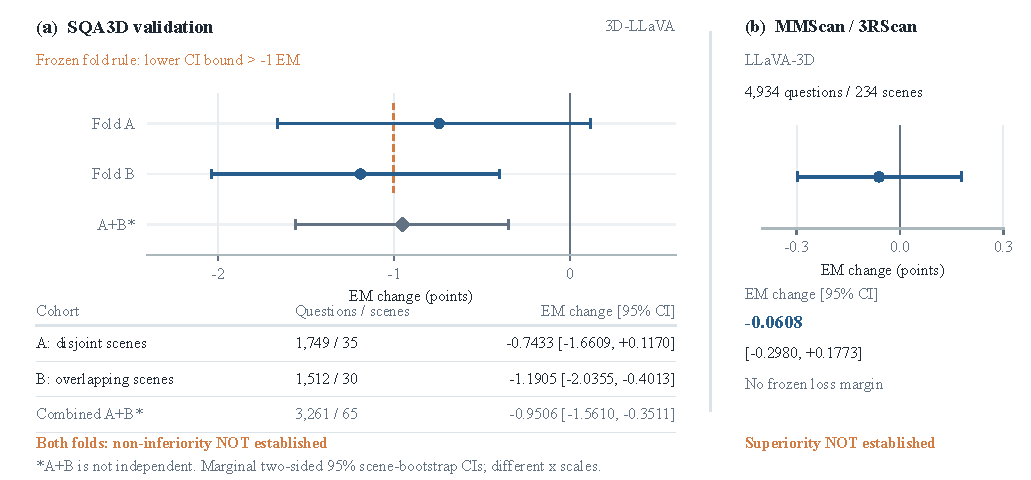
\includegraphics[width=\textwidth]{fig_transfer_effects.pdf}
\caption{\textbf{Quality beyond the original QA comparisons.} SQA3D uses 3D-LLaVA L14/R10; MMScan uses LLaVA-3D L14/R10. Paired EM changes have marginal two-sided 95\% scene intervals. Both SQA3D folds fail the frozen $-1$-EM non-inferiority rule, and the combined row is not an additional independent test. MMScan tests superiority without a tolerated-loss margin. Horizontal scales differ between panels.}
\label{fig:transfereffects}
\end{figure*}

\subsection{Quality Across Tasks and Splits}
Here the comparator changes: we test the selected schedule against the unpruned model, not against cost-matched L2 or L8 pruning. These comparisons assess transfer of task quality, not whether the early--late ordering transfers. Beyond QA, the five-benchmark evaluation includes Scan2Cap dense captioning~\citep{chen2021scan2cap} and referring on ScanRefer~\citep{chen2020scanrefer} and Multi3DRefer~\citep{zhang2023multi3drefer}.
\begin{table}[t]
\centering
\caption{\textbf{Five-benchmark evaluation on 3D-LLaVA.} L14/R10 unless R=20\% is specified. Full sets use official protocols and beam 1. Scan2Cap CIDEr@0.25 scores all 2068 corpus entries, including 2007 with Mask3D predictions and 61 with empty hypotheses. Deltas are computed before rounding. R10 captioning and Multi3DRefer losses are supported by the reported interval analyses; QA and R20 captioning changes remain unresolved.}
\label{tab:five}
\resizebox{\columnwidth}{!}{%
\begin{tabular}{lccccc}
\toprule
Benchmark & Task & Metric & Baseline & GeoGate & $\Delta$ \\
\midrule
ScanQA (4675) & QA & EM@1 & 27.87 & 27.83 & $-0.04$ \\
SQA3D (3519) & QA & EM@1 & 54.82 & 54.90 & $+0.08$ \\
Scan2Cap (2068) & Dense cap. & CIDEr & 79.36 & 76.50 & $-2.85$ \\
\hspace{2em} R=20\% & & CIDEr & 79.36 & 79.06 & $-0.30$ \\
ScanRefer (9508) & Ref. seg. & mIoU & 46.91 & 46.77 & $-0.14$ \\
Multi3DRefer (11120) & Ref. seg. & mIoU & 52.00 & 51.68 & $-0.32$ \\
\bottomrule
\end{tabular}}
\end{table}

The QA point estimates in \Cref{tab:five} do not extend uniformly to other tasks. The supplementary five-endpoint interval table reports R10 QA intervals containing zero. Scan2Cap CIDEr changes by $-2.85$ $[-4.68,-1.11]$ in the original per-endpoint analysis; Multi3DRefer mIoU changes by $-0.32$ $[-0.51,-0.13]$. A separate five-endpoint recomputation finds both decreases significant under post-hoc Holm correction ($p=0.0055$ each), without correcting configuration selection. Its Scan2Cap interval differs from the original interval; the supplement distinguishes these analyses. R20 brings captioning closer to native ($-0.30$, $[-1.53,1.01]$), but the interval still permits a loss and establishes no safe budget. The supplement also reports results for adaptive-onset and unmatched-prompt coverage variants.

\textbf{SQA3D validation.} The fixed 3D-LLaVA L14/R10 configuration fails the quality-preservation test in both frozen folds (\cref{fig:transfereffects}). Together, the folds cover all 3261 validation questions: 1749 questions/35 development-disjoint scenes and 1512 questions/30 development-overlapping scenes. EM changes are $-0.7433$ $[-1.6609,0.1170]$ and $-1.1905$ $[-2.0355,-0.4013]$. Neither fold's one-sided 97.5\% lower bound exceeds the predeclared $-1.0$ EM margin. The combined change of $-0.9506$ $[-1.5610,-0.3511]$ supports a loss under this analysis, but provides no independent-domain confirmation. Post-hoc R20 follow-up leaves both R10 failures unchanged.

\textbf{External 3RScan test.} On MMScan~\citep{lyu2024mmscan}, the L13-to-L14 attention increase appears in all 234 profiled scenes, but its persistence does not predict a quality advantage. On 4934 questions from those scenes, using the checkpoint's required 20 frames, native and L14/R10 EM are 11.0053\% and 10.9445\%: a change of $-0.0608$ $[-0.2980,0.1773]$. CIDEr changes by $-0.2224$ $[-1.6586,1.2359]$. The EM result fails the prespecified superiority test (positive change and one-sided 97.5\% lower bound above zero); it establishes neither degradation nor non-inferiority. No tolerated-loss margin was specified. Across scenes, post-hoc tests find no supported linear or monotonic association between the attention profiles and quality changes (\cref{sec:supp_coupling}).

\subsection{From Analytical Savings to Measured Speed}
\begin{table}[t]
\centering
\caption{\textbf{LLaVA-3D-7B L14/R10 efficiency on one H100.} Each timed setting covers three full-set sessions. Prompt KV estimates storage at decode initialization; allocation delta excludes resident memory. B2/B4 rates divide real-query count by total generation time. Mixed-B4 rates use inverse median allocated query time, whereas their relative result uses native/GeoGate total time. Application time includes preprocessing, transfer, generation, and decoding.}
\label{tab:efficiency}
\resizebox{\columnwidth}{!}{%
\begin{tabular}{lccc}
\toprule
Measure & Baseline & GeoGate & Relative result \\
\midrule
\multicolumn{4}{l}{\emph{Analytical estimates}} \\
LM FLOPs (analytical) & 100\% & 57.9\% & $-42.1\%$ \\
Prompt KV (MiB/query) & 859 & 185 & $-78.5\%$ \\
\multicolumn{4}{l}{\emph{Measured allocation and generation core}} \\
Peak allocation delta (MiB) & 1613 & 1052 & $-34.8\%$ \\
B1 generation median & 145--160 ms & 135--151 ms & $1.061$--$1.072\times$ \\
B2 throughput & 5.46--5.55 q/s & 6.06--6.19 q/s & $1.109$--$1.115\times$ \\
B4 throughput & 6.56--6.68 q/s & 7.69--7.89 q/s & $1.172$--$1.182\times$ \\
Mixed B4 rate & 5.53--5.65 q/s & 6.05--6.18 q/s & $1.088$--$1.091\times$ \\
\multicolumn{4}{l}{\emph{Measured application time}} \\
Application-time reduction & --- & --- & 0.8--1.4\% \\
\bottomrule
\end{tabular}}
\end{table}

Measured application-time savings are much smaller than the analytical LM reduction (\Cref{tab:efficiency}). Across three H100 sessions, generation-core speedups are $1.061\times$--$1.072\times$, while application time decreases by only 0.8--1.4\%. Each B1 session alternates native and GeoGate on identical GPU-resident RGB-D tensors, with CUDA synchronization around generation. Application time covers preprocessing, transfer, generation, and decoding, but not an end-to-end serving system. The same timing runner yields EM changes of $+0.19$ to $+0.28$ and CIDEr changes of $-0.42$ to $-0.61$. All corresponding scene intervals contain zero; this alone does not establish quality equivalence.

Batching improves generation-core throughput by 10.9--11.5\% for same-scene B2 and 17.2--18.2\% for B4; mixed-scene B4 gains are 8.8--9.1\%. Excluding questions with variable outputs gives 8.8--9.2\% gains from recorded batch-time allocations, without rerunning a smaller workload. The mixed-B4 scene bootstrap reweights timings shared across scenes; its coverage under shared-batch and between-session variation remains unvalidated. These workload-specific ratios do not establish general serving-system speedups. The supplement documents output variability, the post-hoc exclusion diagnostic, and original decision criteria.

\textbf{Scope of the quality--cost evidence.} A joint measured comparison requires complete native/official-3DZip/GeoGate sessions with answers and preparation-plus-generation timing, including vision/compression and selection/cache work. The existing separate comparisons cannot form a measured Pareto point. Independent quality preservation requires evaluation beyond the inspected splits. The supplement details the planned OpenEQA-HM3D test~\citep{majumdar2024openeqa}, its frozen scoring endpoint, and unmet asset requirements.
